\chapter{The Uncanny Curve}
In Masahiro Mori's original hypothesis, one can see that if the appearance and the movements of an entity become indistinguishable from humans it is possible for the entity to escape the uncanny valley. Moreover it is even possible that the affinity for an entity which has overcome the uncanny valley exceeds the affinity of entities which have not yet fallen into the uncanny valley. If this hypotheses holds true, it would have major implications for robotics and other scientific fields, as they must strive to design entities whose looks and movements are as similar as possible to that of a human being.\\
On the contrary it may be possible that the uncanny valley rather resembles an uncanny cliff or even an uncanny wall in which the affinity for entities with perfect or near perfect human likeness is in general lower than that of entities that did not fall into the uncanny valley. In this hypothesis, it would not be advantageous to strive for perfect human likeness.

\section{An Uncanny Cliff}
A study by Christoph Bartneck, Takayuki Kanda, Hiroshi Ishiguro and Norihiro Hagita, tried to plot the uncanny valley with particular emphasis on the last ascending section of the curve with more extensive measurements. Furthermore, the referred study also dealt with the question whether highly human-like androids are perceived more likeable when they are being framed as robots. \cite{uncanny_cliff}\\
In the study a framing and a anthropomorphism experiment were conducted. Framing contained three conditions: human, robot and none. Anthropomorphism consisted of four conditions real human, manipulated human, computer graphic and android. Additionally only in the robot framing condition two additional anthropomorphisms were present: humanoid and pet robot. For the experiment only pictures of entities that either exist or which are extremely similar to existing entities were chosen. 
With a questionnaire the human likeness and the likeability of the stimuli was measured.
To ensure the framing conditions of this study three different questionnaires with different framing of the pictures where created. In each different framing of the questionnaire the pictures were either framed as human, robot or only as a face for a neutral comparison. For each anthropomorphism category three different pictures where shown to the participants. 
58 People participated in the study aged between 18 and 41 years. 28 of which were female and 30 were male.
Each of the 18 chosen stimuli was presented to the participants twice. Once with a question about the liking towards the entity, which could be rated on a scale and once with a 7-point semantic differential scales consisting of the values fake/natural, machinelike/human-like, unconscious/conscious, artificial/lifelike, nice/awful, friendly/unfriendly, kind/unkind, and pleasant/unpleasant. This resulted in 36 questions which the participants had to answer on a computer in an randomized order. \cite{uncanny_cliff}\\
The study came to the conclusion that the framing of the entities had no significant influence on the measurements. The pictures where evaluated independently from weather they were labeled as human, robot or face and the labeling did not impact the likeability or human likeness in a negative or positive way.
Moreover the results of the questionnaire showed that anthropomorphism had significant influence on human likeness and likeability. The participants most liked the pictures of toy robots and humanoids. Even though a small upwards trend in likability towards highly human-like entities was noted, not even the pictures of humans reached the affection level of the pictures of toy robots. On the basis of these results the study speculates that even the most human-like androids are not liked as much as toy robots or humanoid. Therefore the study suggests a revised graph of Mori's original graph where there may be small valleys but the main feature is a cliff.
\begin{wrapfigure}{r}{0.5\textwidth} %this figure will be at the right
    \centering
    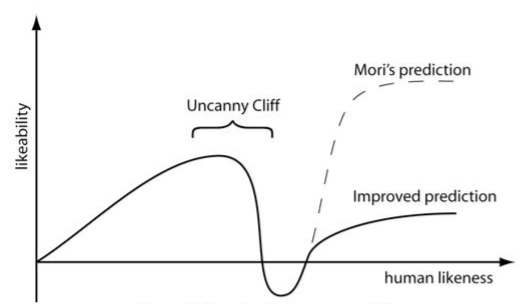
\includegraphics[width=0.5\textwidth]{graphics/uncanny_cliff.png}
    \caption{Hypothesized uncanny cliff.}
    \label{fig:uncannyCliff}
\end{wrapfigure}
In summary, the figure \ref{fig:uncannyCliff} would not describe an uncanny valley but an uncanny cliff.
The results of this study would imply that it is unwise to attempt to build highly human-like entities, since a machine-like robot would be liked more. 
However, the study mentions that in order to further test the hypothesis, more studies need to be conducted with participants from different cultures, as the group of participants in the presented study consisted only of Japanese people, who are stereotypically thought of as being more avid robot-aficionados than other cultures. This could distort the results of the study. \cite{uncanny_cliff}\newpage

\section{An Uncanny Wall}
Both in robotics and in the creation of virtual characters for films and other media, ever-improving technology is allowing progress to be made towards increasing realism. On the basis of these improvements Angela Tinwell and Mark Grimshaw \cite{uncanny_wall} designed a study to furthermore examine and plot the curve of the uncanny valley by using videos of virtual characters.\\
For the study Tinwell et al. \cite{uncanny_wall} choose 100 participants, 92 of them where males and eight females, who where mainly university students from the creative technology field and professionals working within this academic sector and the video game industry. The focus group selected for the study therefore consisted exclusively of people with a lot of knowledge about informatics and game design and art and therefore a lot of exposure and comprehension about the the uncanny valley. Furthermore, significantly more men were selected for the study and no information was given about their age. The method of the study consisted of a web based questionnaire in which the participants had to rate 14 video clips of a selection of virtual characters and one video clip of a real human, which where placed in different settings and engaged in different activities, on a nine-point scale how human-like they perceived the characters and how strange or familiar they perceived the character \cite{uncanny_wall}. The video clips were made up of six photo-realistic characters, five zombie characters, a photo-realistic human-like zombie, three stylised human-like characters including and one real human \cite{uncanny_wall}.\\
In the results of the study there was no single valley to be found. The real person was found to be the most familiar and also the most human-like by the participants. The six photo-realistic characters were found to be very familiar and also very human-like but they could not achieve the ratings of the real person. All zombie-like characters reached very low familiarity and low human-likeness. The three stylised human-like characters had received very different ratings. For example, Mario from Mario and Sonic at the Olympic Games was rated as very familiar but not very human-like, and Lara Croft from Lara Croft Tomb Raider: The Action Adventure was rated as very familiar but only  in the higher midfield of human-likeness. 
The results of the study show that the Uncanny Valley lacks the clarity proposed by Masahiro Mori and paints a more difficult picture with multiple influences affecting the familiarity towards human-like entities felt by participants. The fact that no virtual character could outperform a real person, even though all participants are exposed to the effects of the Uncanny Valley in their everyday lives this study suggests that the Uncanny Valley can be better defined by an Uncanny Wall. Therefore it is not possible to traverse the Uncanny Valley defined by Masahiro Mori. Furthermore the study assumes that with the factor of time audiences do not get used to the Uncanny Valley but that time leads to an increasing discernment on the part of viewers to more small details which do not perfectly resemble real humans. Through this sophistication of discernment the Uncanny Wall rises with time. \cite{uncanny_wall}\\
This study thus paints a new picture of the Uncanny Valley in which it is not possible to overcome it, even with ever-improving technological possibilities. However, it is also worth mentioning that the study's statements should be again validated by conducting the study again with the new possibilities in the development of human-like designs which have emerged in recent times. In such a repeat performance, a larger number of participants should be chosen, who are not all familiar with the subject matter. Finally, when selecting the characters, care should be taken that they are not known to the participants so that the results of the study are not distorted. 

%Subjective Ratings of Robot Video Clips for Human Likeness,
%Familiarity, and Eeriness: An Exploration of the Uncanny Valley
%Karl F. MacDorman
%Vielleicht ein kurzer Vergleich der verschiedenen Ansätze (nicht so klar formuliert wie masahiro mori, jedoch gehen die ansätze zum ende immer stark auseinander im bezug auf das überwinden)







